% ----------------------------------------------------------
% Teste test5_1_e50b128class10_20231212_025758
% ----------------------------------------------------------
\subsubsection{Teste test5_1_e50b128class10_20231212_025758 - AlexNet (Is That a Santa)}

Informações utilizadas para o treinamento.

\begin{table}[ht]
   \centering
   \caption{Treinamento}
   \label{tab:modelos}
   \begin{tabular}{| c | c | }
      \hline 
      \textbf{Informação} & \textbf{Descrição} \\
      \hline \hline 
      Rede & AlexNet \\
      \hline
      Número de épocas & 50\\
      \hline
      Tamanho do lote & 128\\
      \hline
      Taxa inicial & 0.01 \\
      \hline
      Taxa de decaimento & 0.0005 \\
      \hline
      Total de classes & 10\\
      \hline
      Dataset & CIFAR-10\\
      \hline
   \end{tabular} 
\end{table}

Resultados obtidos após treinamento.

\begin{tabular}{lrrrr}
\toprule
  Unnamed: 0 &  precision &  recall &  f1-score &    support \\
\midrule
    airplane &   0.838077 &  0.8540 &  0.845963 &  1000.0000 \\
  automobile &   0.902414 &  0.8970 &  0.899699 &  1000.0000 \\
        bird &   0.750000 &  0.7320 &  0.740891 &  1000.0000 \\
         cat &   0.643821 &  0.6200 &  0.631686 &  1000.0000 \\
        deer &   0.776900 &  0.7870 &  0.781918 &  1000.0000 \\
         dog &   0.715264 &  0.7310 &  0.723046 &  1000.0000 \\
        frog &   0.845709 &  0.8770 &  0.861070 &  1000.0000 \\
       horse &   0.867769 &  0.8400 &  0.853659 &  1000.0000 \\
        ship &   0.883929 &  0.8910 &  0.887450 &  1000.0000 \\
       truck &   0.866000 &  0.8660 &  0.866000 &  1000.0000 \\
    accuracy &   0.809500 &  0.8095 &  0.809500 &     0.8095 \\
   macro avg &   0.808988 &  0.8095 &  0.809138 & 10000.0000 \\
weighted avg &   0.808988 &  0.8095 &  0.809138 & 10000.0000 \\
\bottomrule
\end{tabular}


\begin{figure}[ht]
 \begin{center}
   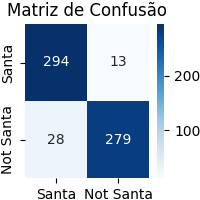
\includegraphics[scale=1]{tests/test5_1_e50b128class10_20231212_025758/confusion_matrix.png}
  \caption{Matriz de Confusão}
  \label{fig:fig03}
 \end{center}
\end{figure}

\begin{figure}[ht]
 \begin{center}
   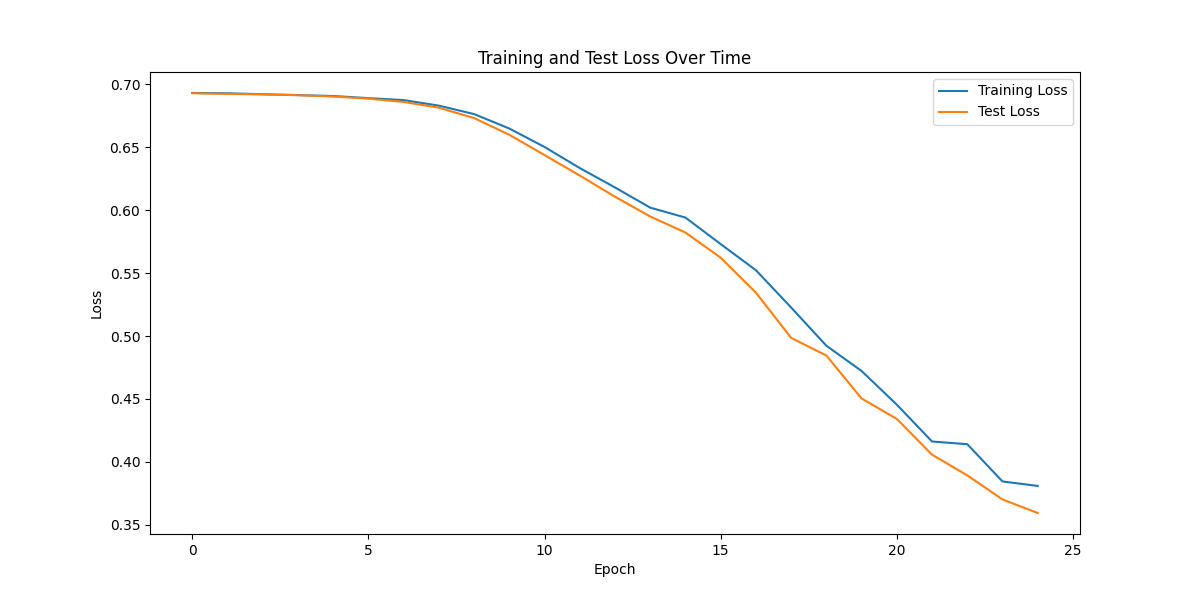
\includegraphics[scale=0.8]{tests/test5_1_e50b128class10_20231212_025758/loss_over_time.png}
  \caption{Gráfico de Perda}
  \label{fig:fig04}
 \end{center}
\end{figure}
